% ----------------------------------------------------------------
% To compile make sure you use pdflatex.  Once latex is installed
% on your system, you can invoke the following command from
% the command-line.
%
% >>> pdflatex hw-template.tex
%
% A successful compilation, will produce the file hw-template.pdf.
%
%
% The remaining part of the file is preamble stuff that you don't
% have to worry about.
%
%
% Head down to where it says "Start here"
% ----------------------------------------------------------------
 
\documentclass[11pt]{article}

\usepackage{fullpage} 
\usepackage{hyperref}
\usepackage{amsmath}
\usepackage{amssymb}
\usepackage{amsthm}
\usepackage{graphicx}
\usepackage{pgf}
\usepackage{tikz}
\usetikzlibrary{arrows,automata}


\newcommand{\question}[2] {\vspace{0.3in}\noindent{\subsection*{Question #1. #2} \vspace{0.15in}}}

\renewcommand{\part}[1] {{\vspace{0.15in}\noindent\textbf (#1)} \vspace{0.10in}}



%  ----------------------------------------------------------------
%                         Start here
% ----------------------------------------------------------------
 
\begin{document}

\title{Assignment \#2} %Replace X with the appropriate number
\author{\Large Gustavo Estrela de Matos\\ %Replace with your name
CSCE 433: Formal Languages and Automata} %If necessary, replace with your course number and title
\date{\today} 

\maketitle


\question{1}{Construct the NFA that accepts the language $\{w \vert w$ contains an odd number of 1's and exactly two 0's$\}$ with exatcly six states.}
First let's build a machine that accepts strings with odd number of 1's:

%\begin{figure}[h]
%\centering
%\fbox{
%    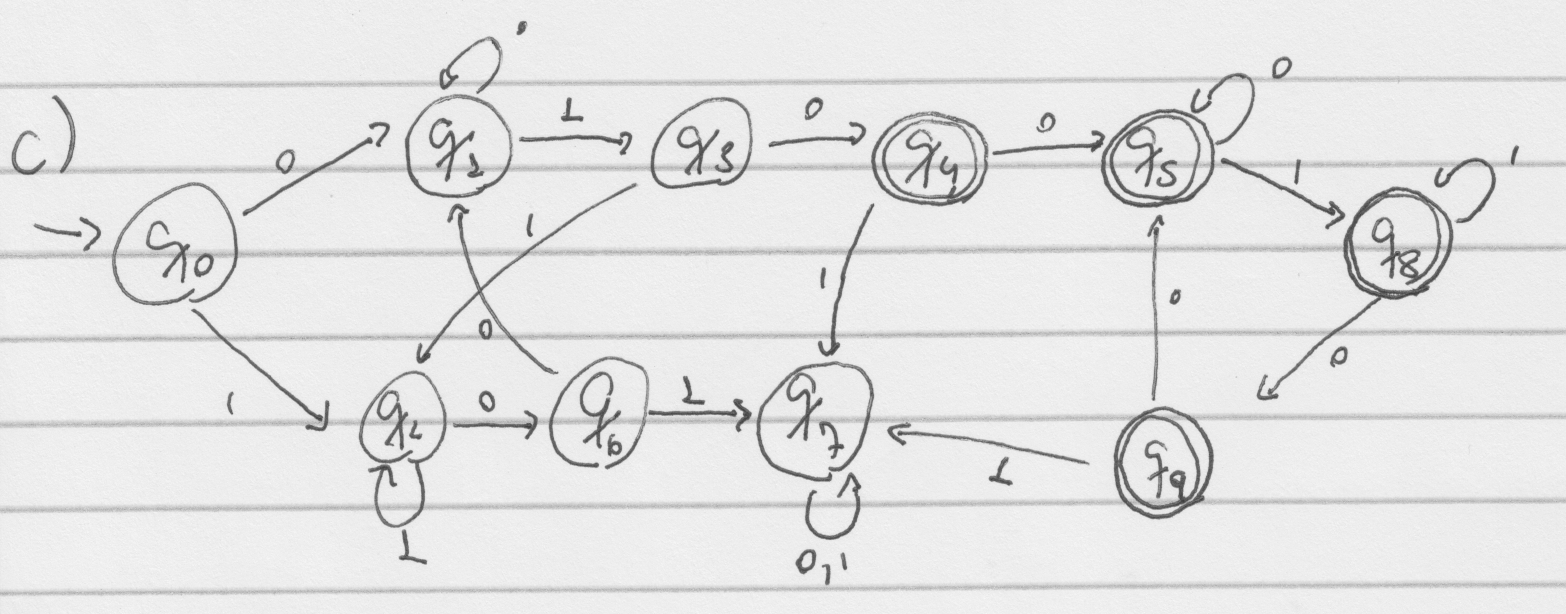
\includegraphics[scale=0.2]{dfa-c.png}
%}
%\end{figure}

Now we build a machine that accepts strings with exactly 2 zeros:

%\begin{figure}[h]
%\centering
%\fbox{
%    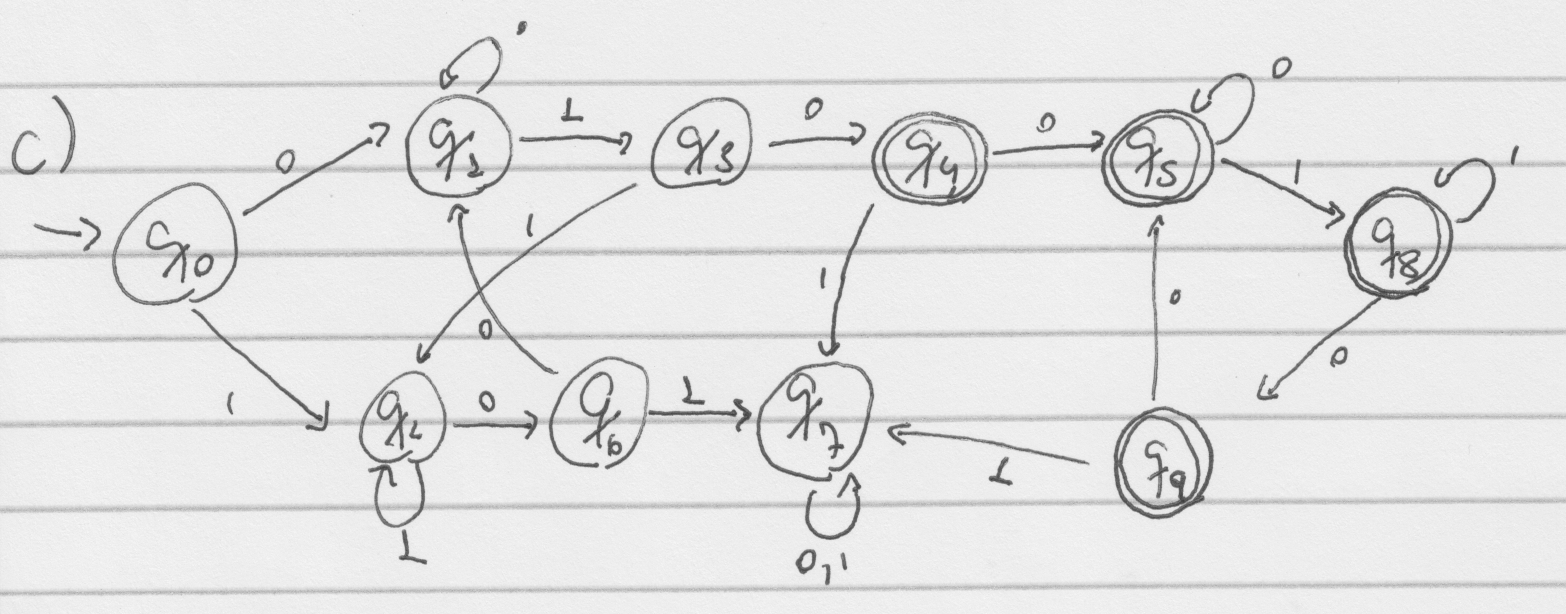
\includegraphics[scale=0.2]{dfa-c.png}
%}
%\end{figure}

Notice that we used 6 states already. Then, since we don't need to keep track of strings that go to state $r_3$, we could simply remove this state, then all the strings with more than 2 zeros would halt on this machine.

Now we can create a new state that goes to both machines without consuming characters of the string:

%\begin{figure}[h]
%\centering
%\fbox{
%    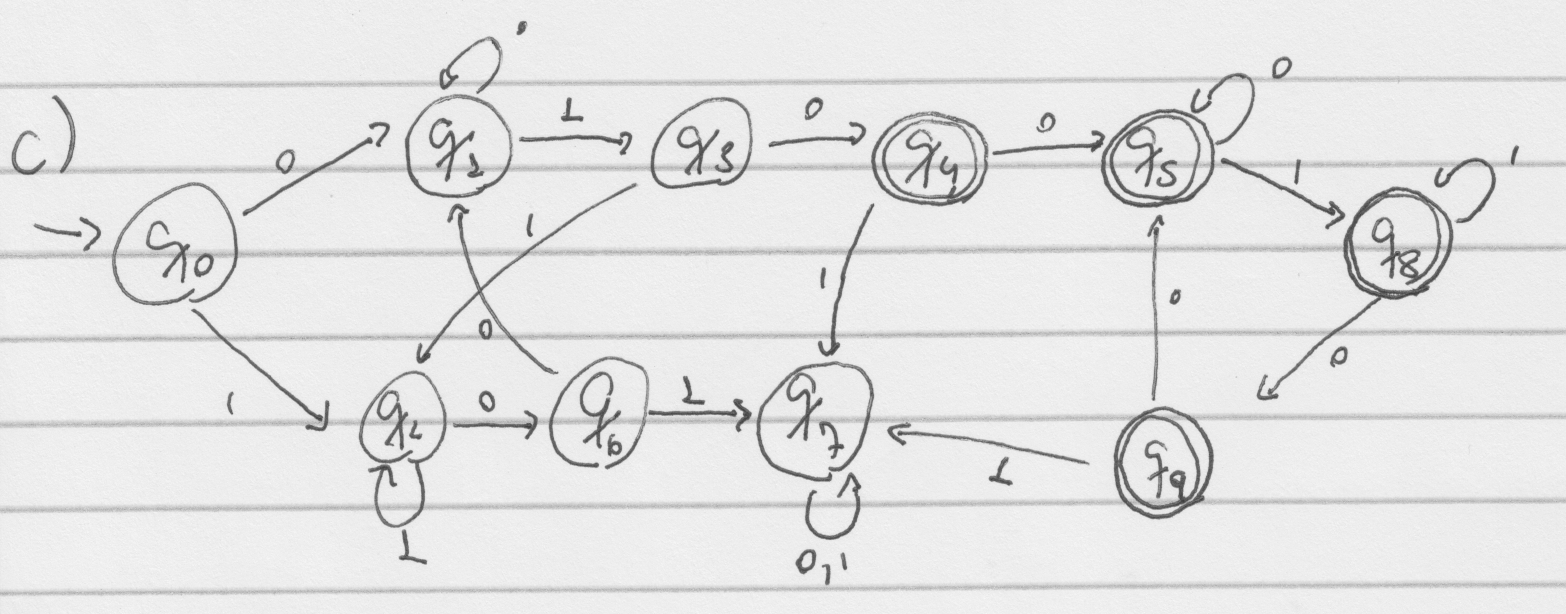
\includegraphics[scale=0.2]{dfa-c.png}
%}
%\end{figure}




\question{2}{Construct an NFA that accepts the set of binary strings that contain both substrings 010 and 101.}
A machine that accepts strings with both substrings $010$ and $101$ has either the substring $010$ or $101$ first, then we could build different machines for both cases:
\begin{itemize}

\item{$010$ and then $101$}

%\begin{figure}[h]
%\centering
%\fbox{
%    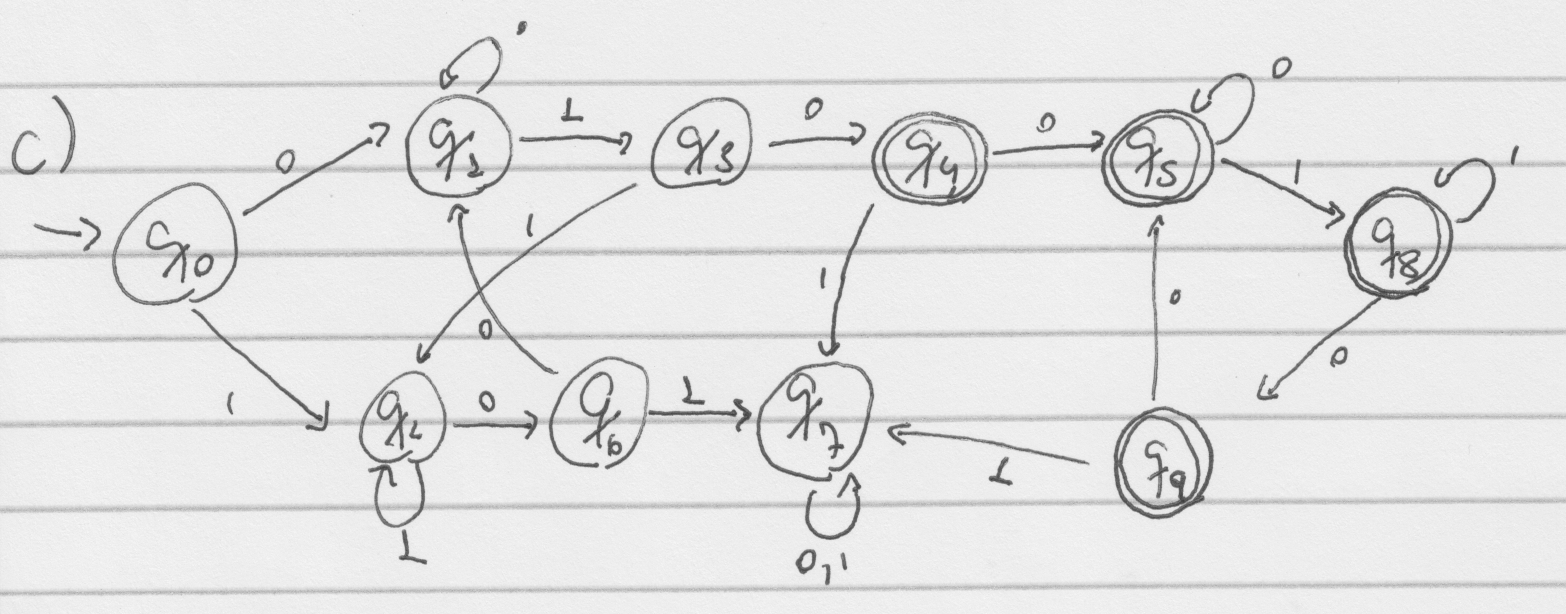
\includegraphics[scale=0.2]{dfa-c.png}
%}
%\end{figure}

Notice that the machine consider the case in which $010$ and $101$ overlaps.

\item{$101$ and then $010$}
%\begin{figure}[h]
%\centering
%\fbox{
%    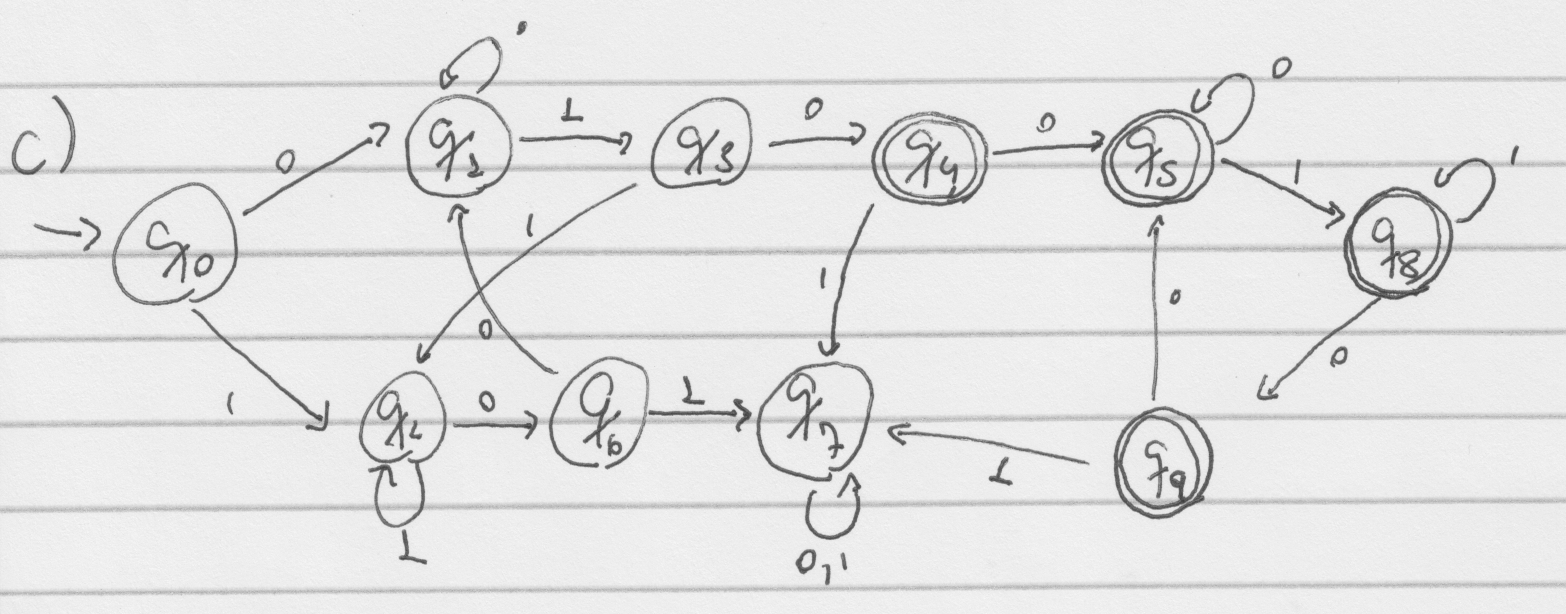
\includegraphics[scale=0.2]{dfa-c.png}
%}
%\end{figure}

\end{itemize}



\question{3}{Convert the NFA below to a DFA}
%\begin{figure}[h]
%\centering
%\fbox{
%    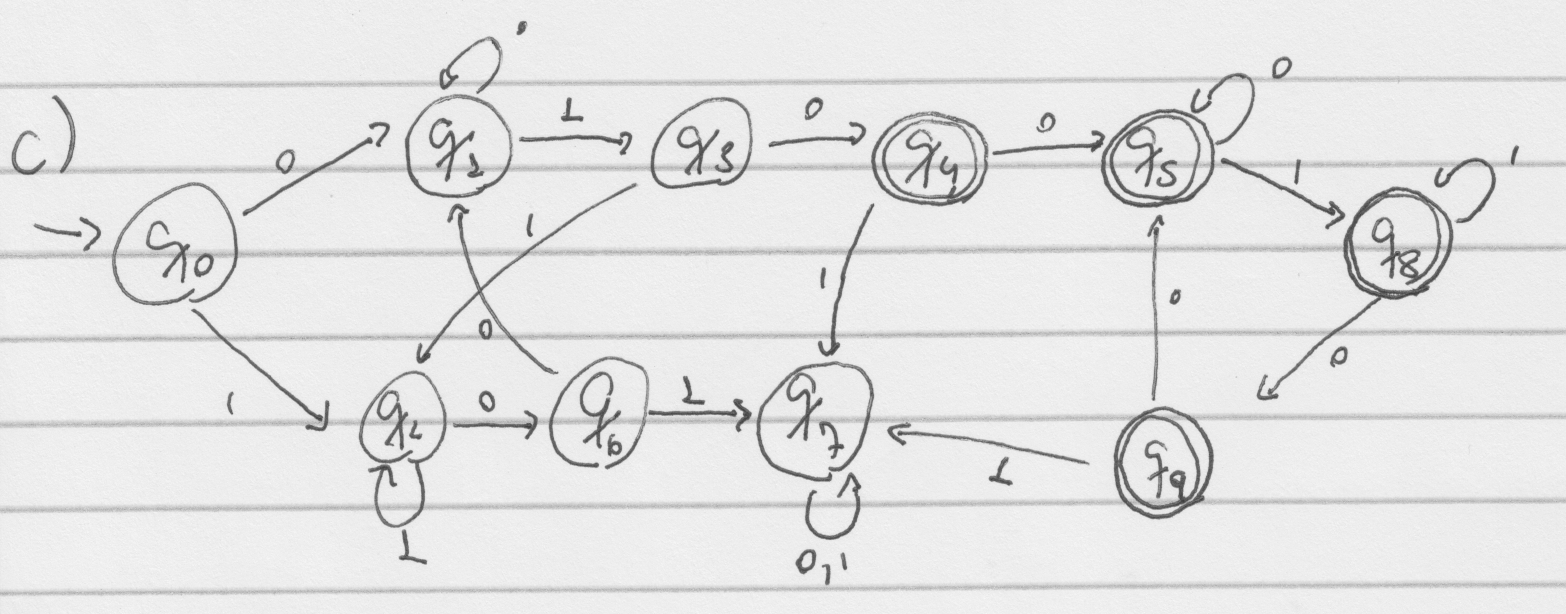
\includegraphics[scale=0.2]{dfa-c.png}
%}
%\end{figure}
To solve this question we are going to use the same algorithm used to proove that $\epsilon$-NFAs are equivalent to DFAs. We are going to call this NFA $N = (Q, \Sigma, \delta, q, F)$ and build an equivalent DFA $M = (Q', \Sigma, \delta', q', F')$ such that $q' = C_{\epsilon}(0) = \{0, 1\}$; $\delta': \mathcal{P}(Q) \times \Sigma$ where $\delta'(R, a) = \bigcup \limits_{r \in R}^{} C_{\epsilon}(\delta(r, a))$ as it follows:

\begin{itemize}
\item{Start with the initial state}
%\begin{figure}[h]
%\centering
%\fbox{
%    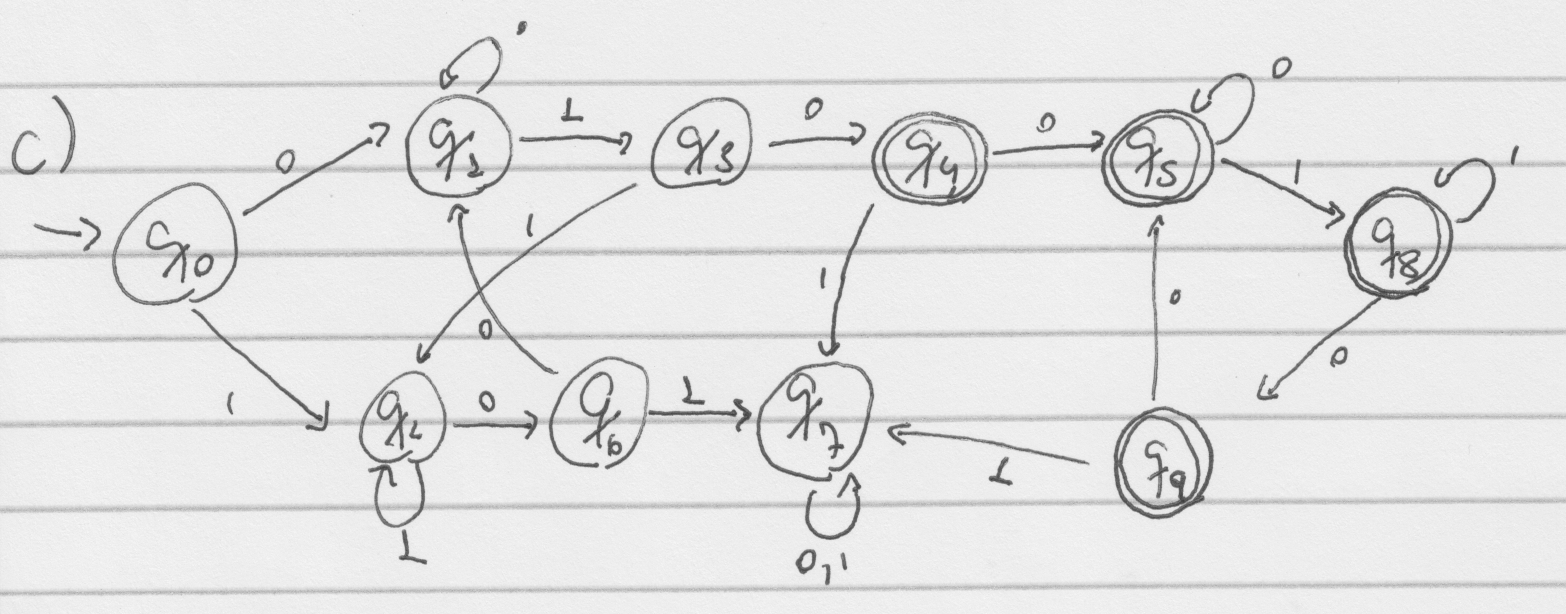
\includegraphics[scale=0.2]{dfa-c.png}
%}
%\end{figure}


\item{Calculate the transitions of $\{0, 1\}$}

$\delta'(\{0, 1\}, a) = C_{\epsilon}(1) \cup \emptyset = \{1\}$\\
$\delta'(\{0, 1\}, b) = \emptyset \cup C_{\epsilon}(2) = \{0, 1, 2\}$\\

%\begin{figure}[h]
%\centering
%\fbox{
%    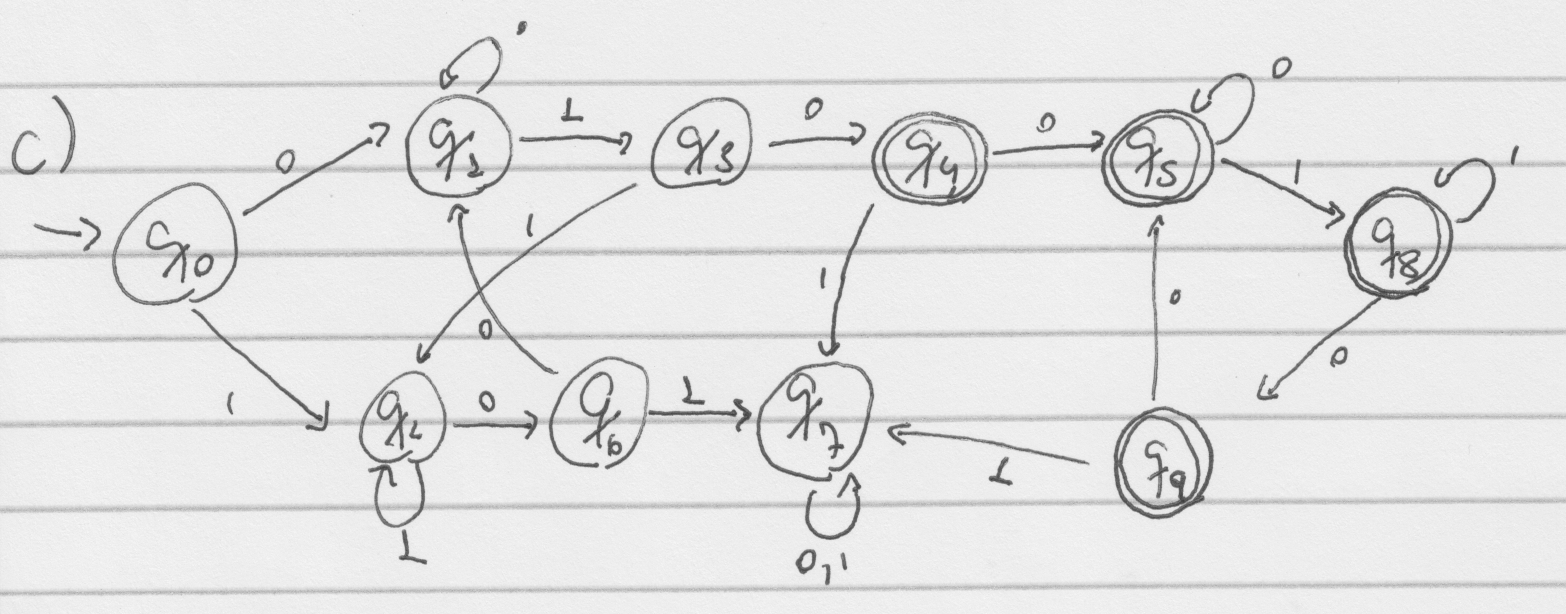
\includegraphics[scale=0.2]{dfa-c.png}
%}
%\end{figure}


\item{Calculate the transitions of \{1\} and \{0, 1, 2\}}

$\delta'(\{1\}, a) = \emptyset$\\
$\delta'(\{1\}, b) = C_{\epsilon}(2) = \{0, 1, 2\}$\\
$\delta'(\{0, 1, 2\}, a) = C_{\epsilon}(1) \cup \emptyset \cup C_{\epsilon}(3)= \{1, 3\}$\\
$\delta'(\{0, 1, 2\}, b) = \emptyset \cup C_{\epsilon}(2) \cup \emptyset = \{0, 1, 2\}$\\

%\begin{figure}[h]
%\centering
%\fbox{
%    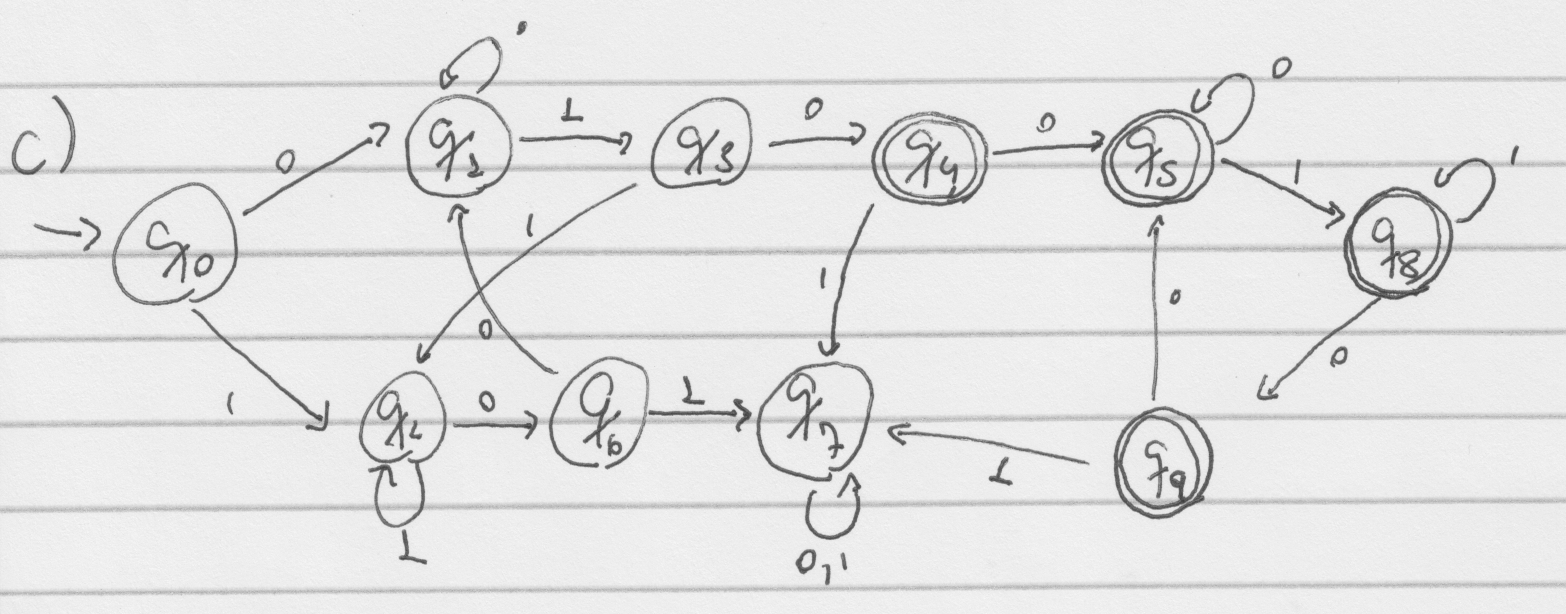
\includegraphics[scale=0.2]{dfa-c.png}
%}
%\end{figure}


\item{Calculate the transitions of \{1, 3\}}


\end{itemize}

\end{document}

